\documentclass{article} % For LaTeX2e
\usepackage{iclr2025_conference,times}

\usepackage{hyperref}
\usepackage{url}
\usepackage{booktabs}
\usepackage{graphicx}
\usepackage{subcaption}
\usepackage{amsmath}
\usepackage{microtype}

\title{Detecting LLM-Generated Student Essays with Transformer Fine-Tuning and Robustness Analysis}

\author{Joseph Souaiby \quad Huzaifah Wasim \\
Georgia Institute of Technology 
}

\newcommand{\fix}{\marginpar{FIX}}
\newcommand{\new}{\marginpar{NEW}}

\iclrfinalcopy
\begin{document}

\maketitle

% ─────────────────────────────────────────────
\section{Introduction}
% ─────────────────────────────────────────────




% ─────────────────────────────────────────────
\section{Related Work}
% ─────────────────────────────────────────────



% ─────────────────────────────────────────────
\section{Problem Decomposition \& Detailed Technical Approach}
% ─────────────────────────────────────────────



\subsection{Data Processing}

\textbf{Kaggle dataset.} We used the "LLM Detect AI Generated Text" dataset \citep{thite2026kaggle}
which contained 27{,}278 labeled essays after preprocessing. It was processed using whitespace normalization,
removal of duplicate essays (1{,}861 removed), and filtering of essays shorter than 50
characters. We applied stratified splits: 80\% train (21{,}822), 10\% validation (2{,}728),
10\% test (2{,}728).

\textbf{RAID dataset.} For OOD evaluation, we used the RAID benchmark \citep{dugan2024raid}
loaded from HuggingFace. We sampled a balanced subset of 10{,}000
samples (5{,}900 human, 4{,}100 AI) from multiple AI models, providing a realistic
cross-domain test bench. RAID was chosen over HC3/TURINGBENCH because it includes generated text from a wider variety of AI models and writing domains, providing a harder and more realistic OOD test. The processing of the subset was done using the same method employed for the Kaggle dataset

\subsection{Baseline: TF-IDF + Linear Classifiers}

Essays were vectorized using TF-IDF with the following configuration: 50{,}000 maximum features,
unigram and bigram tokens, sublinear TF scaling ($\text{tf} = 1 + \log(\text{tf})$), minimum
document frequency of 5, maximum document frequency of 95\%. We trained two classifiers:
Logistic Regression (L2, $C=1$, lbfgs solver) and LinearSVC ($C=1.0$,
max\_iter=2000), both with balanced class weights.



\subsection{Evaluation Procedure}

All models were evaluated on the same Kaggle test set (2{,}728 essays) for in-domain
performance, and on the balanced RAID subset (10{,}000 texts) for OOD performance. Metrics used are:
Accuracy, F1-score, Recall, Precision, and AUROC. Confusion matrices and
ROC curves are generated for all experiments. 

% ─────────────────────────────────────────────
\section{Experiments and Results}
% ─────────────────────────────────────────────

\subsection{Datasets}

Our established data pipeline covers two datasets. The Kaggle dataset is the primary
training and in-domain evaluation source whereas RAID serves as the OOD evaluation benchmark. Both
datasets are fully processed using the methods described in the data processing section. Table~\ref{tab:data} summarizes key statistics.

\begin{table}[h]
    \centering
    \caption{Dataset statistics used in all experiments.}
    \label{tab:data}
    \small
    \begin{tabular}{lcccc}
        \toprule
        Dataset & Total & Human & AI & Usage \\
        \midrule
        Kaggle (train) & 21{,}822 & 12{,}878 & 8{,}944 & Baseline \& model training \\
        Kaggle (val)   &  2{,}728 &  1{,}610 & 1{,}118 & Hyperparameter selection \\
        Kaggle (test)  &  2{,}728 &  1{,}610 & 1{,}118 & In-domain evaluation \\
        RAID (subset)  & 10{,}000 &  5{,}900 & 4{,}100 & OOD evaluation \\
        \bottomrule
    \end{tabular}
\end{table}

\subsection{Exploratory Data Analysis}

EDA on the Kaggle dataset as seen in Fig \ref{fig:teaser} and Fig \ref{fig:vocab_metrics} reveals clear differences
between human and AI essays. AI generated essays are on average longer, with 360 words vs. 280 words for humans, use more formal and repetitive vocabulary leading to a lower type-token ratio of 0.55 vs. 0.60 for humans, and favour institutional bigrams such as "electoral college",
"important role", "United States". Human essays use more varied, personal vocabulary
such as "people", "car", "like", "driving". These differences motivate TF-IDF as a discriminative
baseline, while also indicating the risk of exploiting dataset-specific artifacts rather than
genuinely generalisable features.

\begin{figure}[h!]
    \centering
    \begin{subfigure}[b]{0.3\textwidth}
        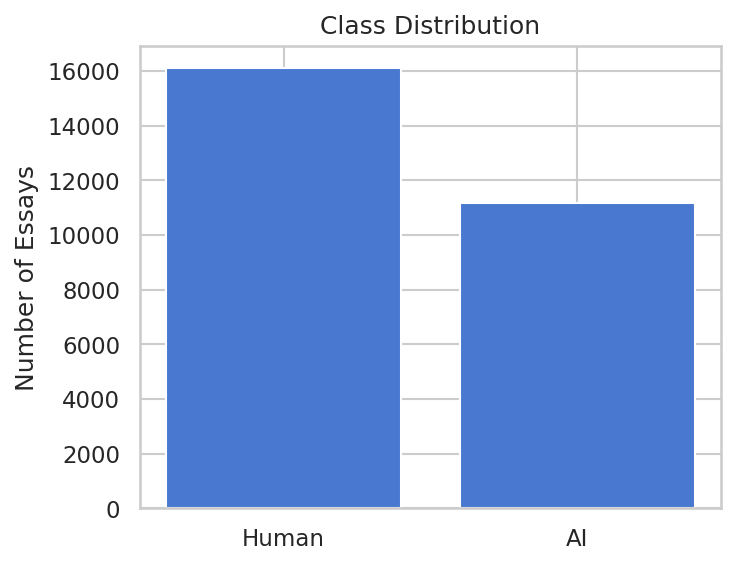
\includegraphics[width=\textwidth]{results/eda_kaggle/kaggle_class_distribution.png}
        \caption{Class distribution.}
    \end{subfigure}
    \hfill
    \begin{subfigure}[b]{0.6\textwidth}
        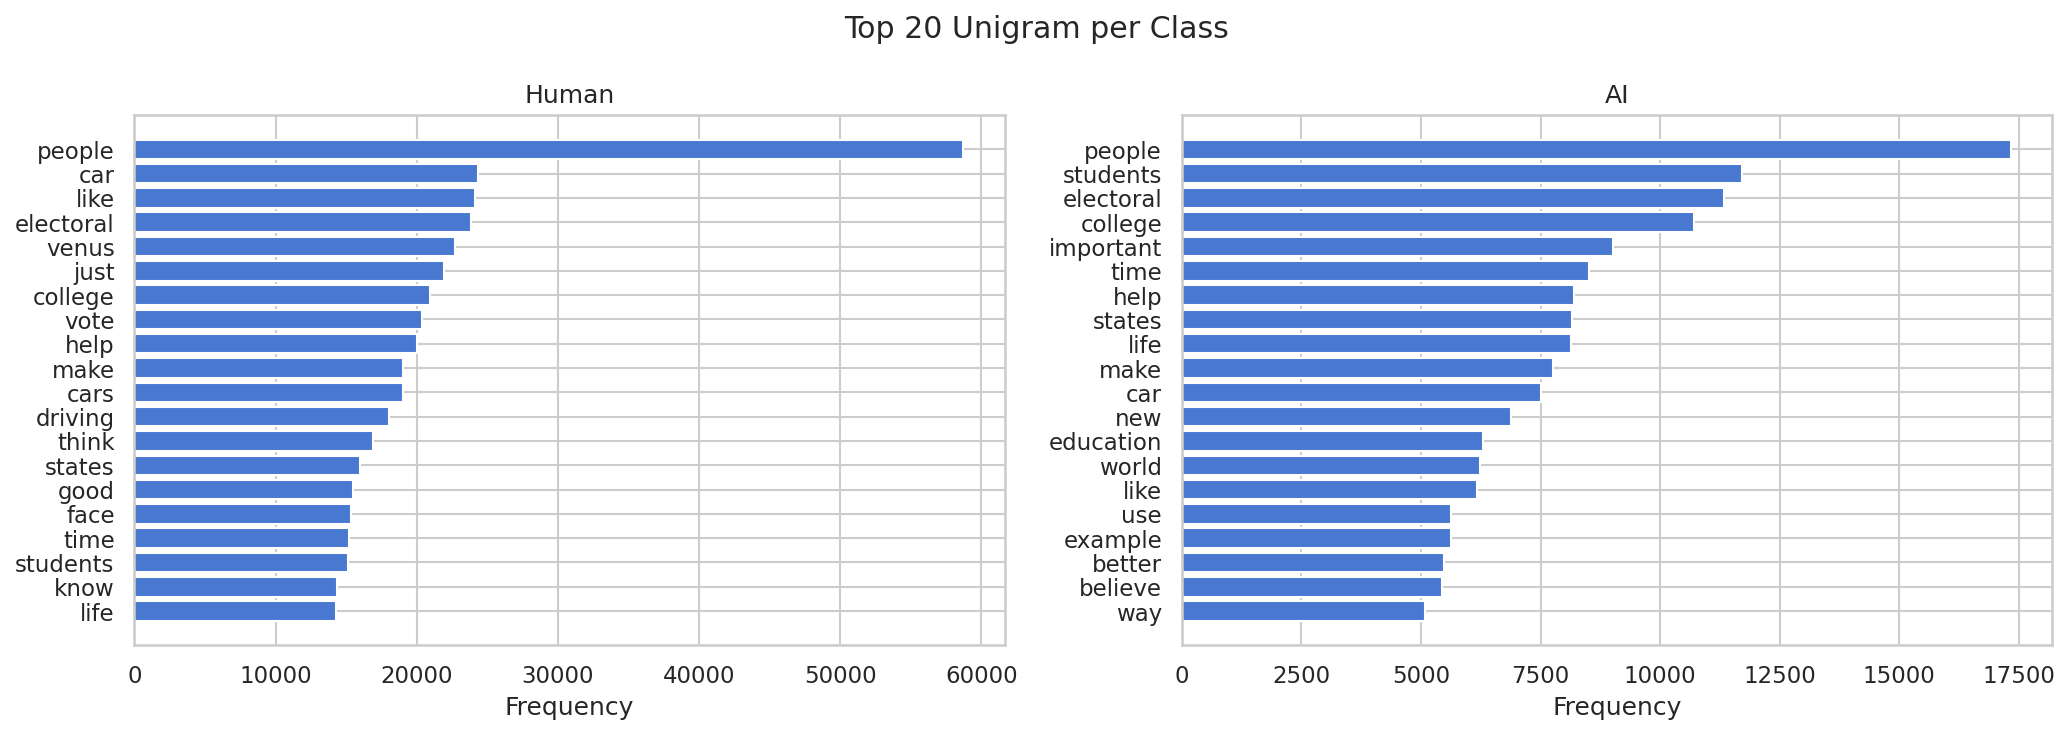
\includegraphics[width=\textwidth]{results/eda_kaggle/kaggle_unigram.png}
        \caption{Top unigrams per class.}
    \end{subfigure}
    \caption{Exploratory data analysis on the Kaggle dataset. AI-generated essays show distinct
    vocabulary patterns: more formal, repetitive language (lower type-token ratio) and
    longer average word length compared to human essays.}
    \label{fig:teaser}
\end{figure}

\begin{figure}[h!]
    \centering
    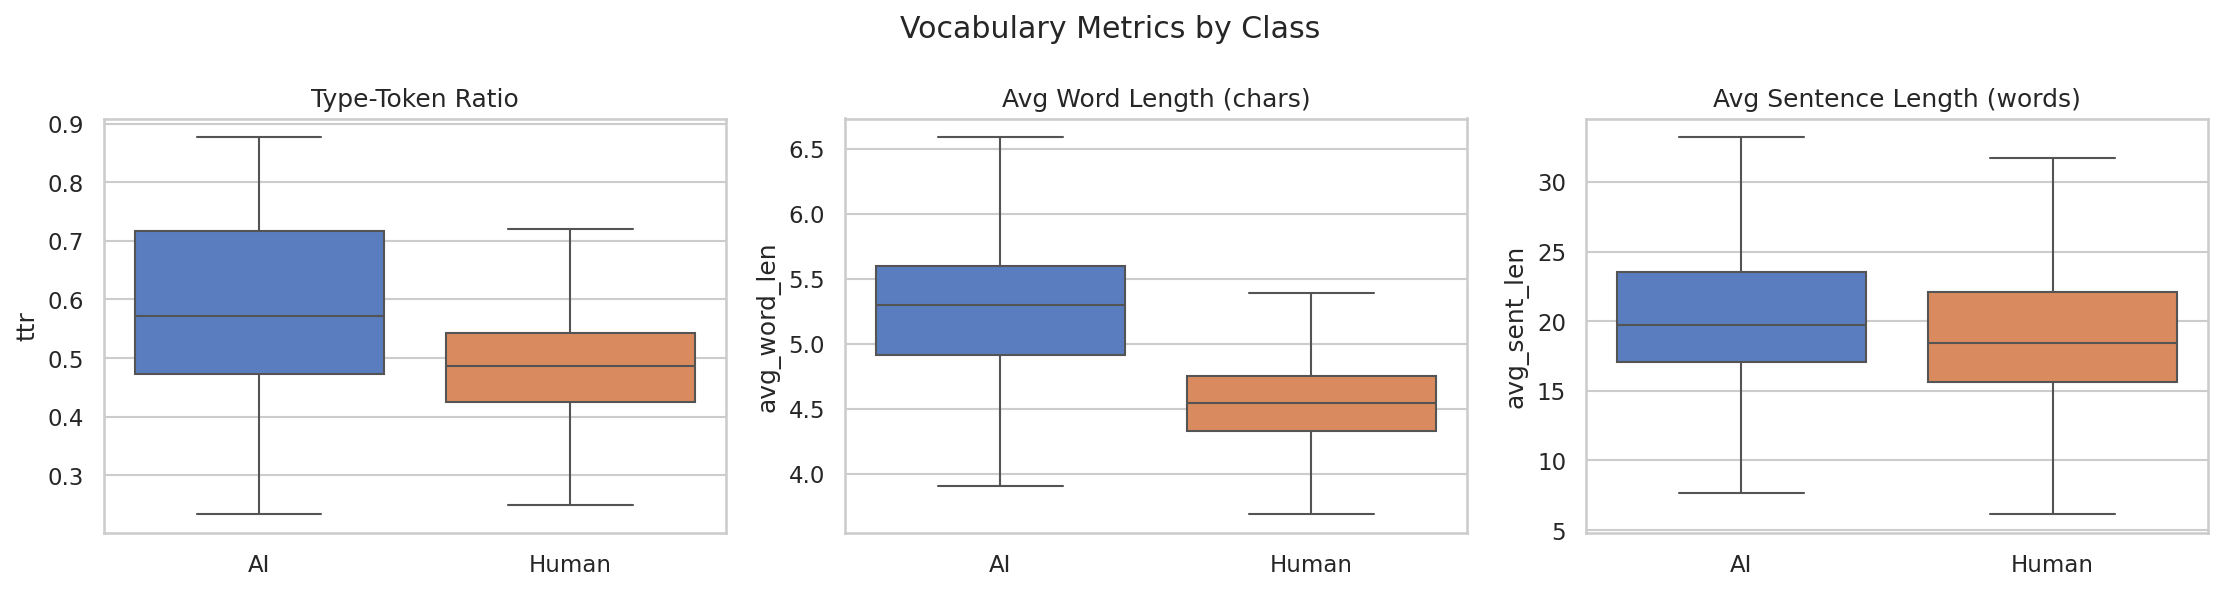
\includegraphics[width=0.8\textwidth]{results/eda_kaggle/kaggle_vocab_metrics.png}
    \caption{Vocabulary metrics per class (Kaggle)}
    \label{fig:vocab_metrics}
\end{figure}

Fig \ref{fig:raid-eda} and Fig \ref{fig:raid_vocab_metrics} show the corresponding EDA on the RAID subset. Two key factors that can be seen in the metrics reported
justify the OOD failure reported in the results section. First, the top unigrams per
class in RAID are substantially different from Kaggle topic-specific terms in kaggle vocabulary, indicating that the lexical patterns learned on the Kaggle dataset do
are not transferable. Second, while vocabulary richness metrics (type-token ratio, average word length)
show similar between-class trends in both datasets, their absolute distributions differ enough
that TF-IDF weights trained on the kaggle dataset are ill-suited for RAID. Together
these observations confirm that the Kaggle baseline's near-perfect accuracy reflects
dataset-specific artifacts rather than generalizable patterns.

\begin{figure}[h]
    \centering
    \begin{subfigure}[b]{0.3\textwidth}
        
\includegraphics[width=\textwidth]{results/eda_raid/raid_class_distribution.png}
        \caption{Class distribution (RAID).}
    \end{subfigure}
    \hfill
    \begin{subfigure}[b]{0.6\textwidth}
        
\includegraphics[width=\textwidth]{results/eda_raid/raid_unigram.png}
        \caption{Top unigrams per class (RAID).}
    \end{subfigure}
    \caption{EDA on the RAID OOD dataset. The top unigrams are markedly different from those
    in Kaggle (Figure~\ref{fig:teaser}b), and the absolute vocabulary metric distributions
    shift, causing TF-IDF features trained on Kaggle to be systematically miscalibrated.}
    \label{fig:raid-eda}
\end{figure}

\begin{figure}[h]
    \centering
    
\includegraphics[width=0.8\textwidth]{results/eda_raid/raid_vocab_metrics.png}
    \caption{Vocabulary metrics per class (RAID).}
    \label{fig:raid_vocab_metrics}
\end{figure}

\newpage
\subsection{Baseline Results}

Table~\ref{tab:results} reports in-domain (Kaggle) and OOD (RAID) performance for both baselines.
Figure~\ref{fig:kaggle-results} shows confusion matrices and ROC curves on Kaggle, Figure~\ref{fig:raid-results}
shows the corresponding OOD results.

\begin{table}[h]
    \centering
    \caption{Baseline performance on the Kaggle test set (in-domain) and RAID (OOD).}
    \label{tab:results}
    \small
    \begin{tabular}{lcccccc}
        \toprule
        & \multicolumn{3}{c}{\textbf{Kaggle (in-domain)}} & \multicolumn{3}{c}{\textbf{RAID (OOD)}} \\
        \cmidrule(lr){2-4} \cmidrule(lr){5-7}
        Model & Acc.\ (\%) & F1 & AUROC & Acc.\ (\%) & F1 & AUROC \\
        \midrule
        TF-IDF + LogReg   & 99.89 & 0.989 & 1.00 & 40.86 & 0.580 & 0.66 \\
        TF-IDF + LinearSVC & 99.92 & 0.997 & 1.00 & 40.90 & 0.580 & 0.66 \\
        \bottomrule
    \end{tabular}
\end{table}

Both TF-IDF baselines achieve almost performance on the in-domain Kaggle test set
with Accuracy = 99.8\% and AUROC = 1.00, consistent with the fact that this dataset has LLM-generated essays which contain strong lexical patterns. However,
both models suffer a huge drop when evaluated on RAID and fall to 41\% accuracy, which is 
close to or below random chance. The RAID confusion matrices show that
nearly all human essays are misclassified as AI-generated, suggesting the models have latched
onto Kaggle-specific vocabulary patterns rather than learning generalizable patterns.
This OOD failure strongly motivates the use of transformer-based models, which may capture
deeper semantic features less tied to surface-level vocabulary.

\begin{figure}[t]
    \centering
    \begin{subfigure}[b]{0.28\textwidth}
        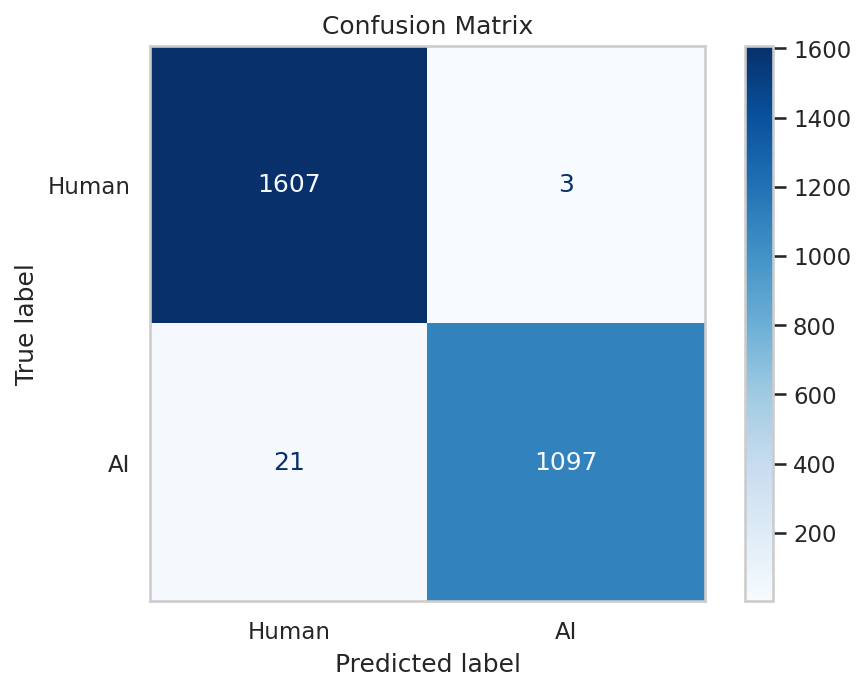
\includegraphics[width=\textwidth]{results/log_reg/confusion_matrix.png}
        \caption{Log-Reg CM}
    \end{subfigure}
    \begin{subfigure}[b]{0.23\textwidth}
        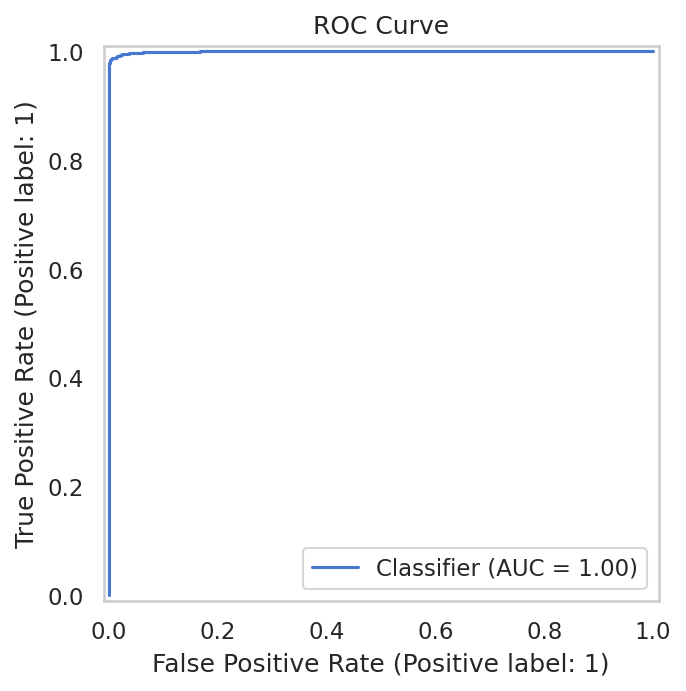
\includegraphics[width=\textwidth]{results/log_reg/roc_auc_plot.png}
        \caption{Log-Reg ROC}
    \end{subfigure}
    \begin{subfigure}[b]{0.28\textwidth}
        
\includegraphics[width=\textwidth]{results/SVM/confusion_matrix.png}
        \caption{LinearSVC CM}
    \end{subfigure}
    \begin{subfigure}[b]{0.23\textwidth}
        
\includegraphics[width=\textwidth]{results/SVM/roc_auc_plot.png}
        \caption{LinearSVC ROC}
    \end{subfigure}
    \caption{In-domain baseline results on the Kaggle test set. Both baselines achieve near-perfect
    discrimination (AUROC = 1.00).}
    \label{fig:kaggle-results}
\end{figure}

\begin{figure}[h!]
    \centering
    \begin{subfigure}[b]{0.28\textwidth}
        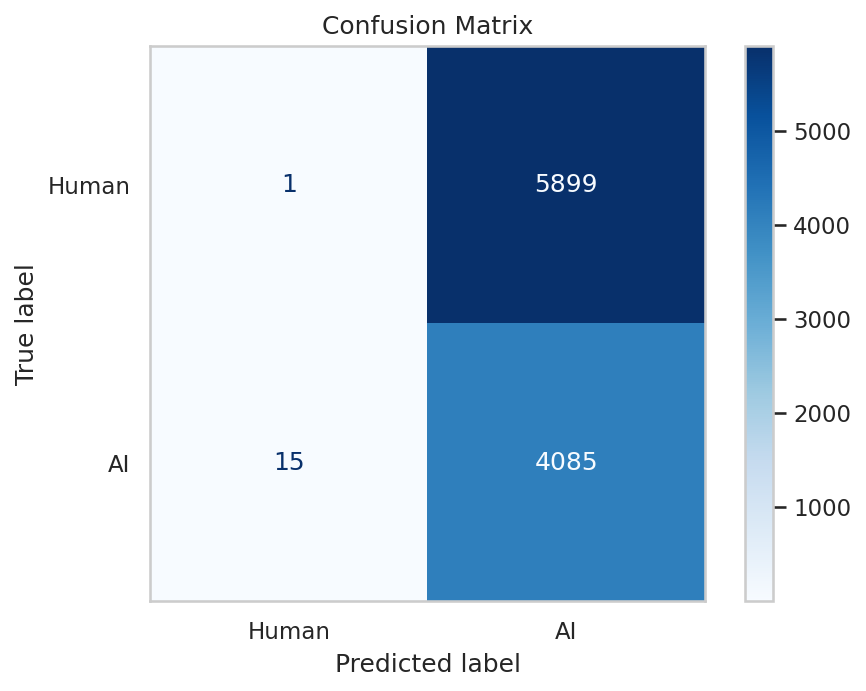
\includegraphics[width=\textwidth]{results/raid_log_reg/confusion_matrix.png}
        \caption{Log-Reg CM}
    \end{subfigure}
    \begin{subfigure}[b]{0.23\textwidth}
        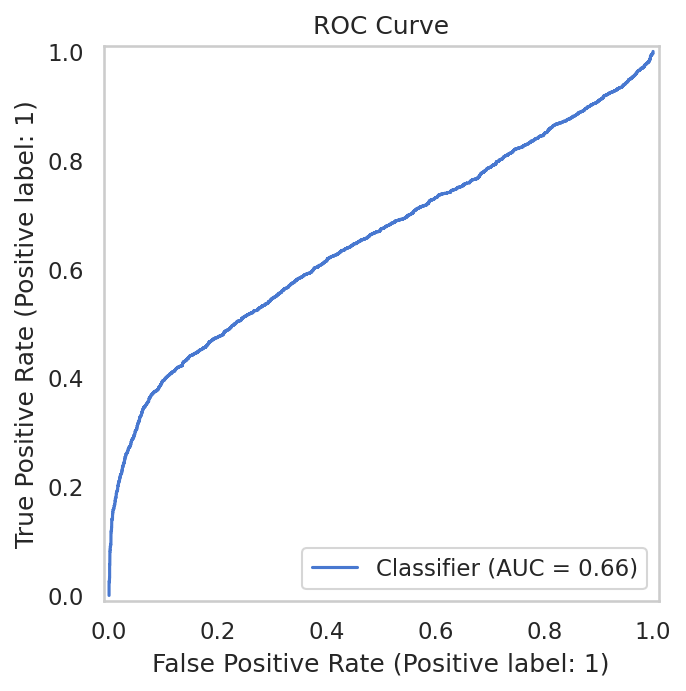
\includegraphics[width=\textwidth]{results/raid_log_reg/roc_auc_plot.png}
        \caption{Log-Reg ROC}
    \end{subfigure}
    \begin{subfigure}[b]{0.28\textwidth}
        
\includegraphics[width=\textwidth]{results/raid_SVM/confusion_matrix.png}
        \caption{LinearSVC CM}
    \end{subfigure}
    \begin{subfigure}[b]{0.23\textwidth}
        
\includegraphics[width=\textwidth]{results/raid_SVM/roc_auc_plot.png}
        \caption{LinearSVC ROC}
    \end{subfigure}
    \caption{OOD baseline results on RAID. Both baselines collapse to $\sim$41\% accuracy,
    misclassifying nearly all human essays as AI-generated.}
    \label{fig:raid-results}
\end{figure}

\newpage
% ─────────────────────────────────────────────
\section{Next Steps}
% ─────────────────────────────────────────────



% ─────────────────────────────────────────────
\newpage
\bibliography{references}
\bibliographystyle{iclr2025_conference}

\end{document}
